\documentclass[12pt,a4paper]{article}
\usepackage[utf8]{vietnam}
\usepackage{amsmath,amssymb}
\usepackage[a4paper,left=2cm,right=1.8cm,top=1.8cm,bottom=1.8cm]{geometry}
\usepackage{tikz}
\usepackage{array,tabularx,longtable}
\usepackage{enumitem}
\setlength{\parindent}{0pt}
\setlength{\parskip}{3pt}
\linespread{1.15}
\pagestyle{plain}

% Phương án trắc nghiệm: 4 phương án trên 1 dòng / 2 dòng / mỗi phương án 1 dòng
\newcommand{\bonpa}[4]{\par\noindent\begin{tabularx}{\linewidth}{@{\hspace{0.6cm}}XXXX@{}}
\textbf{A.} #1 & \textbf{B.} #2 & \textbf{C.} #3 & \textbf{D.} #4\end{tabularx}\par}
\newcommand{\haipa}[4]{\par\noindent\begin{tabularx}{\linewidth}{@{\hspace{0.6cm}}XX@{}}
\textbf{A.} #1 & \textbf{B.} #2\\ \textbf{C.} #3 & \textbf{D.} #4\end{tabularx}\par}
\newcommand{\motpa}[4]{\par\hspace*{0.6cm}\textbf{A.} #1\par\hspace*{0.6cm}\textbf{B.} #2\par
\hspace*{0.6cm}\textbf{C.} #3\par\hspace*{0.6cm}\textbf{D.} #4\par}
\newcommand{\cau}[1]{\par\medskip\textbf{Câu #1.}~}
\newcommand{\bai}[2]{\par\medskip\textbf{Bài #1} \textit{(#2)}.~}
\newcommand{\y}[1]{\par\hspace*{0.6cm}#1}
\newcommand{\phan}[1]{\par\bigskip{\large\textbf{#1}}\par\smallskip}
\setlength{\extrarowheight}{2pt}

\begin{document}
% ===================== ĐỀ SỐ 3 =====================
\noindent
\begin{minipage}[t]{0.38\linewidth}\centering
TRƯỜNG THCS \dotfill\\[2pt]
\textbf{ĐỀ SỐ 3}
\end{minipage}\hfill
\begin{minipage}[t]{0.6\linewidth}\centering
\textbf{ĐỀ KIỂM TRA GIỮA HỌC KÌ I}\\
\textbf{NĂM HỌC 2026 -- 2027}\\
\textbf{MÔN: TOÁN 7} -- Sách \textit{Kết nối tri thức với cuộc sống}\\
\textit{Thời gian làm bài: 90 phút (không kể thời gian giao đề)}
\end{minipage}

\medskip
Họ và tên: \dotfill\ Lớp: \makebox[2cm]{\dotfill}\ Số báo danh: \makebox[2.5cm]{\dotfill}
\phan{A. TRẮC NGHIỆM (3,0 điểm)}
\textbf{Phần I. Câu trắc nghiệm nhiều phương án lựa chọn} \textit{(1,0 điểm)}. Thí sinh trả lời từ câu 1 đến câu 4. Mỗi câu hỏi thí sinh chỉ chọn một phương án.
\cau{1} Phân số nào sau đây biểu diễn số hữu tỉ $-0{,}75$?
\bonpa{$\dfrac{3}{4}$}{$\dfrac{-3}{4}$}{$\dfrac{-7}{5}$}{$\dfrac{-4}{3}$}
\cau{2} Kết quả của phép tính $\left(\dfrac{1}{2}\right)^{6}:\left(\dfrac{1}{2}\right)^{2}$ là
\bonpa{$\left(\dfrac{1}{2}\right)^{3}$}{$\left(\dfrac{1}{2}\right)^{4}$}{$\left(\dfrac{1}{2}\right)^{8}$}{$\left(\dfrac{1}{2}\right)^{12}$}
\cau{3} Làm tròn số $3{,}14159$ đến hàng phần trăm ta được
\bonpa{$3{,}14$}{$3{,}15$}{$3{,}1$}{$3{,}142$}
\cau{4} Trong một tam giác vuông, hai góc nhọn
\bonpa{bằng nhau.}{bù nhau.}{phụ nhau.}{kề bù.}

\medskip\textbf{Phần II. Câu trắc nghiệm đúng sai} \textit{(1,0 điểm)}. Trong mỗi ý a), b), c), d) ở câu 5, thí sinh chọn đúng hoặc sai.
\cau{5} Xét tính đúng, sai của các khẳng định sau:
\y{a) $\left(-\dfrac{1}{2}\right)^{4}=\dfrac{1}{16}$.}
\y{b) $3^{2}\cdot 3^{3}=3^{6}$.}
\y{c) $\left(2^{3}\right)^{2}=2^{6}$.}
\y{d) $\left(-\dfrac{2}{3}\right)^{0}=0$.}

\medskip\textbf{Phần III. Câu trắc nghiệm trả lời ngắn} \textit{(1,0 điểm)}. Thí sinh trả lời từ câu 6 đến câu 9.
\cau{6} Tính $\dfrac{-5}{6}+\dfrac{1}{3}$ (viết kết quả dưới dạng số thập phân).
\cau{7} Tìm $x$, biết $x:\dfrac{2}{3}=-\dfrac{9}{4}$ (viết kết quả dưới dạng số thập phân).
\cau{8} Đường thẳng $c$ cắt hai đường thẳng song song $a$ và $b$. Biết một góc tạo bởi $c$ và $a$ bằng $72^\circ$. Tính số đo góc đồng vị với góc đó (đơn vị: độ).
\cau{9} Cho $\triangle MNP=\triangle HIK$, biết $\widehat{M}=50^\circ$, $\widehat{I}=70^\circ$. Tính số đo $\widehat{P}$ (đơn vị: độ).
\phan{B. TỰ LUẬN (7,0 điểm)}
\bai{1}{1,0 điểm} Tính (hợp lí nếu có thể):
\y{a) $\dfrac{15}{34}+\dfrac{7}{21}+\dfrac{19}{34}-1\dfrac{15}{17}+\dfrac{2}{3}$;}
\y{b) $(-2)^{3}\cdot\left(\dfrac{1}{2}\right)^{2}+\left(\dfrac{3}{4}-\dfrac{1}{4}\right):\dfrac{1}{8}$.}
\bai{2}{1,5 điểm} Tìm $x$, biết:
\y{a) $x-\dfrac{3}{5}=\dfrac{1}{2}$;}
\y{b) $\dfrac{2}{3}x+\dfrac{1}{4}=\dfrac{5}{12}$;}
\y{c) $(2x-1)^{3}=-8$.}
\bai{3}{1,0 điểm} Một mảnh vườn hình chữ nhật có chiều dài $12{,}5$ m, chiều rộng bằng $\dfrac{4}{5}$ chiều dài.
\y{a) Tính chu vi và diện tích mảnh vườn.}
\y{b) Người ta dùng $\dfrac{3}{5}$ diện tích mảnh vườn để trồng rau. Tính diện tích phần đất trồng rau.}
\bai{4}{1,5 điểm} Cho hình vẽ bên, biết $a\perp c$, $b\perp c$, đường thẳng $d$ cắt $a$, $b$ lần lượt tại $M$, $N$ và $\widehat{M_1}=120^\circ$.
\begin{center}
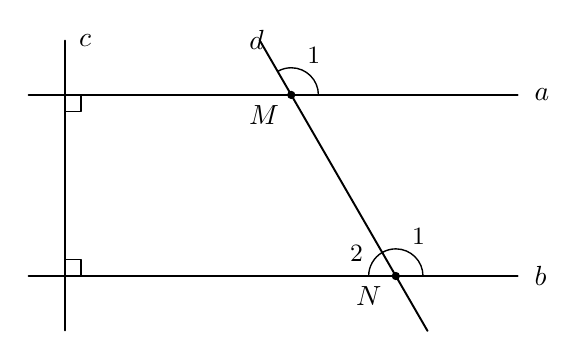
\begin{tikzpicture}[scale=1.15,line cap=round,line join=round]
  \draw[line width=0.7pt] (0.000,-0.600) -- (0.000,2.600);
  \draw[line width=0.7pt] (-0.400,2.000) -- (5.000,2.000);
  \draw[line width=0.7pt] (-0.400,0.000) -- (5.000,0.000);
  \node[anchor=west,inner sep=1pt] at (0.120,2.600) {$c$};
  \node[anchor=west,inner sep=1pt] at (5.150,2.000) {$a$};
  \node[anchor=west,inner sep=1pt] at (5.150,0.000) {$b$};
  \draw[line width=0.5pt] (0.180,2.000) -- (0.180,1.820) -- (0.000,1.820);
  \draw[line width=0.5pt] (0.180,0.000) -- (0.180,0.180) -- (0.000,0.180);
  \draw[line width=0.7pt] (2.150,2.606) -- (4.005,-0.606);
  \node[anchor=west,inner sep=1pt] at (2.000,2.606) {$d$};
  \fill (2.500,2.000) circle (1.3pt);
  \node[anchor=center,inner sep=1pt] at (2.200,1.780) {$M$};
  \fill (3.655,0.000) circle (1.3pt);
  \node[anchor=center,inner sep=1pt] at (3.355,-0.220) {$N$};
  \draw[line width=0.5pt] (2.800,2.000) arc[start angle=0,end angle=120,radius=0.300];
  \node[anchor=center,inner sep=1pt] at (2.750,2.433) {{\small 1}};
  \draw[line width=0.5pt] (3.955,0.000) arc[start angle=0,end angle=120,radius=0.300];
  \node[anchor=center,inner sep=1pt] at (3.905,0.433) {{\small 1}};
  \draw[line width=0.5pt] (3.505,0.260) arc[start angle=120,end angle=180,radius=0.300];
  \node[anchor=center,inner sep=1pt] at (3.222,0.250) {{\small 2}};
\end{tikzpicture}
\end{center}
\y{a) Vì sao $a\parallel b$?}
\y{b) Tính số đo $\widehat{N_1}$.}
\y{c) Tính số đo $\widehat{N_2}$.}
\bai{5}{1,5 điểm} Cho đoạn thẳng $AB$. Lấy hai điểm $C$ và $D$ nằm khác phía đối với đường thẳng $AB$ sao cho $CA=DA$ và $CB=DB$.
\y{a) Chứng minh $\triangle ACB=\triangle ADB$.}
\y{b) Chứng minh $AB$ là tia phân giác của $\widehat{CAD}$.}
\y{c) Biết $\widehat{CAD}=100^\circ$, $\widehat{ACB}=95^\circ$. Tính số đo $\widehat{CBD}$.}
\bai{6}{0,5 điểm} Tìm $x$, biết: $\dfrac{x+1}{2025}+\dfrac{x+2}{2024}=\dfrac{x+3}{2023}+\dfrac{x+4}{2022}$.

\bigskip\begin{center}\textbf{--------- HẾT ---------}\\
\textit{Giáo viên coi kiểm tra không giải thích gì thêm.}\end{center}

\newpage
\begin{center}{\large\textbf{HƯỚNG DẪN CHẤM -- ĐỀ SỐ 3}}\end{center}
\phan{A. TRẮC NGHIỆM (3,0 điểm)}
\textbf{Phần I.} Mỗi câu trả lời đúng được 0,25 điểm.

\begin{tabular}{|l|*{4}{>{\centering\arraybackslash}p{2cm}|}}\hline
Câu & 1 & 2 & 3 & 4 \\ \hline
Đáp án & \textbf{B} & \textbf{B} & \textbf{A} & \textbf{C} \\ \hline
\end{tabular}

\textbf{Phần II.} Mỗi ý trả lời đúng được 0,25 điểm.

\begin{tabular}{|l|*{4}{>{\centering\arraybackslash}p{2cm}|}}\hline
Câu 5 & a) & b) & c) & d) \\ \hline
Đáp án & \textbf{Đúng} & \textbf{Sai} & \textbf{Đúng} & \textbf{Sai} \\ \hline
\end{tabular}

\textbf{Phần III.} Mỗi câu trả lời đúng được 0,25 điểm.

\begin{tabular}{|l|*{4}{>{\centering\arraybackslash}p{2cm}|}}\hline
Câu & 6 & 7 & 8 & 9 \\ \hline
Đáp án & \textbf{$-$0,5} & \textbf{$-$1,5} & \textbf{72} & \textbf{60} \\ \hline
\end{tabular}

\phan{B. TỰ LUẬN (7,0 điểm)}
\begin{longtable}{|>{\bfseries}c|p{0.76\linewidth}|>{\centering\arraybackslash}p{1.3cm}|}\hline
Bài & \multicolumn{1}{c|}{\textbf{Nội dung}} & \textbf{Điểm} \\ \hline\endhead
1a & \rule{0pt}{4ex}$=\left(\dfrac{15}{34}+\dfrac{19}{34}\right)+\left(\dfrac{1}{3}+\dfrac{2}{3}\right)-\dfrac{32}{17}=1+1-\dfrac{32}{17}$\rule[-2.4ex]{0pt}{0pt} & 0,25 \\ \hline
 & \rule{0pt}{4ex}$=\dfrac{34}{17}-\dfrac{32}{17}=\dfrac{2}{17}$\rule[-2.4ex]{0pt}{0pt} & 0,25 \\ \hline
1b & \rule{0pt}{4ex}$=(-8)\cdot\dfrac{1}{4}+\dfrac{1}{2}:\dfrac{1}{8}=-2+\dfrac{1}{2}\cdot 8$\rule[-2.4ex]{0pt}{0pt} & 0,25 \\ \hline
 & $=-2+4=2$ & 0,25 \\ \hline
2a & \rule{0pt}{4ex}$x=\dfrac{1}{2}+\dfrac{3}{5}=\dfrac{5}{10}+\dfrac{6}{10}$\rule[-2.4ex]{0pt}{0pt} & 0,25 \\ \hline
 & \rule{0pt}{4ex}$x=\dfrac{11}{10}$. Vậy $x=\dfrac{11}{10}$.\rule[-2.4ex]{0pt}{0pt} & 0,25 \\ \hline
2b & \rule{0pt}{4ex}$\dfrac{2}{3}x=\dfrac{5}{12}-\dfrac{1}{4}=\dfrac{5}{12}-\dfrac{3}{12}=\dfrac{1}{6}$\rule[-2.4ex]{0pt}{0pt} & 0,25 \\ \hline
 & \rule{0pt}{4ex}$x=\dfrac{1}{6}:\dfrac{2}{3}=\dfrac{1}{4}$. Vậy $x=\dfrac{1}{4}$.\rule[-2.4ex]{0pt}{0pt} & 0,25 \\ \hline
2c & $(2x-1)^{3}=(-2)^{3}$ nên $2x-1=-2$ & 0,25 \\ \hline
 & \rule{0pt}{4ex}$2x=-1$, $x=-\dfrac{1}{2}$. Vậy $x=-\dfrac{1}{2}$.\rule[-2.4ex]{0pt}{0pt} & 0,25 \\ \hline
3a & \rule{0pt}{4ex}Chiều rộng mảnh vườn: $12{,}5\cdot\dfrac{4}{5}=10$ (m).\rule[-2.4ex]{0pt}{0pt} & 0,25 \\ \hline
 & Chu vi mảnh vườn: $2\cdot(12{,}5+10)=45$ (m). & 0,25 \\ \hline
 & Diện tích mảnh vườn: $12{,}5\cdot 10=125$ ($\mathrm{m}^{2}$). & 0,25 \\ \hline
3b & \rule{0pt}{4ex}Diện tích phần đất trồng rau: $125\cdot\dfrac{3}{5}=75$ ($\mathrm{m}^{2}$).\rule[-2.4ex]{0pt}{0pt} & 0,25 \\ \hline
4a & Ta có $a\perp c$ và $b\perp c$ & 0,25 \\ \hline
 & nên $a\parallel b$ (hai đường thẳng phân biệt cùng vuông góc với đường thẳng thứ ba). & 0,25 \\ \hline
4b & Vì $a\parallel b$ nên $\widehat{N_1}=\widehat{M_1}$ (hai góc đồng vị) & 0,25 \\ \hline
 & Do đó $\widehat{N_1}=120^\circ$. & 0,25 \\ \hline
4c & $\widehat{N_1}$ và $\widehat{N_2}$ là hai góc kề bù nên $\widehat{N_1}+\widehat{N_2}=180^\circ$ & 0,25 \\ \hline
 & $\widehat{N_2}=180^\circ-120^\circ=60^\circ$. & 0,25 \\ \hline
5 & Vẽ hình, ghi GT – KL đúng. \newline \textit{(Hình vẽ ở cuối hướng dẫn chấm)} & 0,25 \\ \hline
5a & Xét $\triangle ACB$ và $\triangle ADB$ có: $CA=DA$ (gt); $CB=DB$ (gt); $AB$ là cạnh chung. & 0,25 \\ \hline
 & Do đó $\triangle ACB=\triangle ADB$ (c.c.c). & 0,25 \\ \hline
5b & Từ câu a suy ra $\widehat{CAB}=\widehat{DAB}$ (hai góc tương ứng). Mà tia $AB$ nằm giữa hai tia $AC$, $AD$ nên $AB$ là tia phân giác của $\widehat{CAD}$. & 0,25 \\ \hline
5c & \rule{0pt}{4ex}$\widehat{CAB}=\dfrac{100^\circ}{2}=50^\circ$. Trong $\triangle ACB$: $\widehat{ABC}=180^\circ-50^\circ-95^\circ=35^\circ$.\rule[-2.4ex]{0pt}{0pt} & 0,25 \\ \hline
 & Vì $\triangle ACB=\triangle ADB$ nên $\widehat{ABD}=\widehat{ABC}=35^\circ$. Do đó $\widehat{CBD}=35^\circ+35^\circ=70^\circ$. & 0,25 \\ \hline
6 & \rule{0pt}{4ex}Cộng thêm $1$ vào mỗi phân số ta được $\dfrac{x+2026}{2025}+\dfrac{x+2026}{2024}=\dfrac{x+2026}{2023}+\dfrac{x+2026}{2022}$ \newline hay $(x+2026)\cdot\left(\dfrac{1}{2025}+\dfrac{1}{2024}-\dfrac{1}{2023}-\dfrac{1}{2022}\right)=0$.\rule[-2.4ex]{0pt}{0pt} & 0,25 \\ \hline
 & \rule{0pt}{4ex}Vì $\dfrac{1}{2025}<\dfrac{1}{2023}$ và $\dfrac{1}{2024}<\dfrac{1}{2022}$ nên biểu thức trong ngoặc khác $0$. Do đó $x+2026=0$, $x=-2026$.\rule[-2.4ex]{0pt}{0pt} & 0,25 \\ \hline
\end{longtable}
\textit{Lưu ý: Học sinh làm cách khác đúng vẫn cho điểm tối đa theo thang điểm tương ứng. Bài hình không vẽ hình hoặc vẽ hình sai không chấm phần tương ứng.}

\textbf{Hình vẽ bài 5:}
\begin{center}
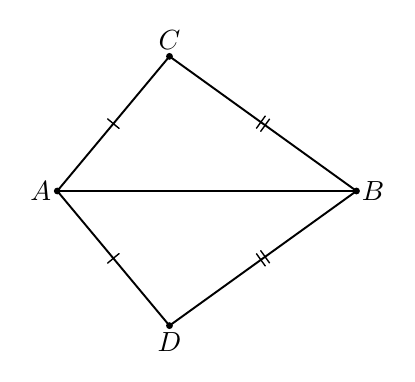
\begin{tikzpicture}[scale=0.95,line cap=round,line join=round]
  \draw[line width=0.7pt] (0.000,0.000) -- (4.000,0.000);
  \draw[line width=0.7pt] (0.000,0.000) -- (1.500,1.800);
  \draw[line width=0.7pt] (1.500,1.800) -- (4.000,0.000);
  \draw[line width=0.7pt] (0.000,0.000) -- (1.500,-1.800);
  \draw[line width=0.7pt] (1.500,-1.800) -- (4.000,0.000);
  \draw[line width=0.5pt] (0.827,0.836) -- (0.673,0.964);
  \draw[line width=0.5pt] (0.673,-0.964) -- (0.827,-0.836);
  \draw[line width=0.5pt] (2.663,0.839) -- (2.780,1.002);
  \draw[line width=0.5pt] (2.720,0.798) -- (2.837,0.961);
  \draw[line width=0.5pt] (2.780,-1.002) -- (2.663,-0.839);
  \draw[line width=0.5pt] (2.837,-0.961) -- (2.720,-0.798);
  \fill (0.000,0.000) circle (1.3pt);
  \node[anchor=center,inner sep=1pt] at (-0.220,0.000) {$A$};
  \fill (4.000,0.000) circle (1.3pt);
  \node[anchor=center,inner sep=1pt] at (4.220,0.000) {$B$};
  \fill (1.500,1.800) circle (1.3pt);
  \node[anchor=center,inner sep=1pt] at (1.500,2.020) {$C$};
  \fill (1.500,-1.800) circle (1.3pt);
  \node[anchor=center,inner sep=1pt] at (1.500,-2.020) {$D$};
\end{tikzpicture}
\end{center}

\end{document}
